\documentclass{standalone}
\usepackage{tikz}
\usetikzlibrary{patterns, positioning}
\usepackage[sfdefault]{ClearSans} %% option 'sfdefault' activates Clear Sans as the default text font
\usepackage[T1]{fontenc}

\begin{document}
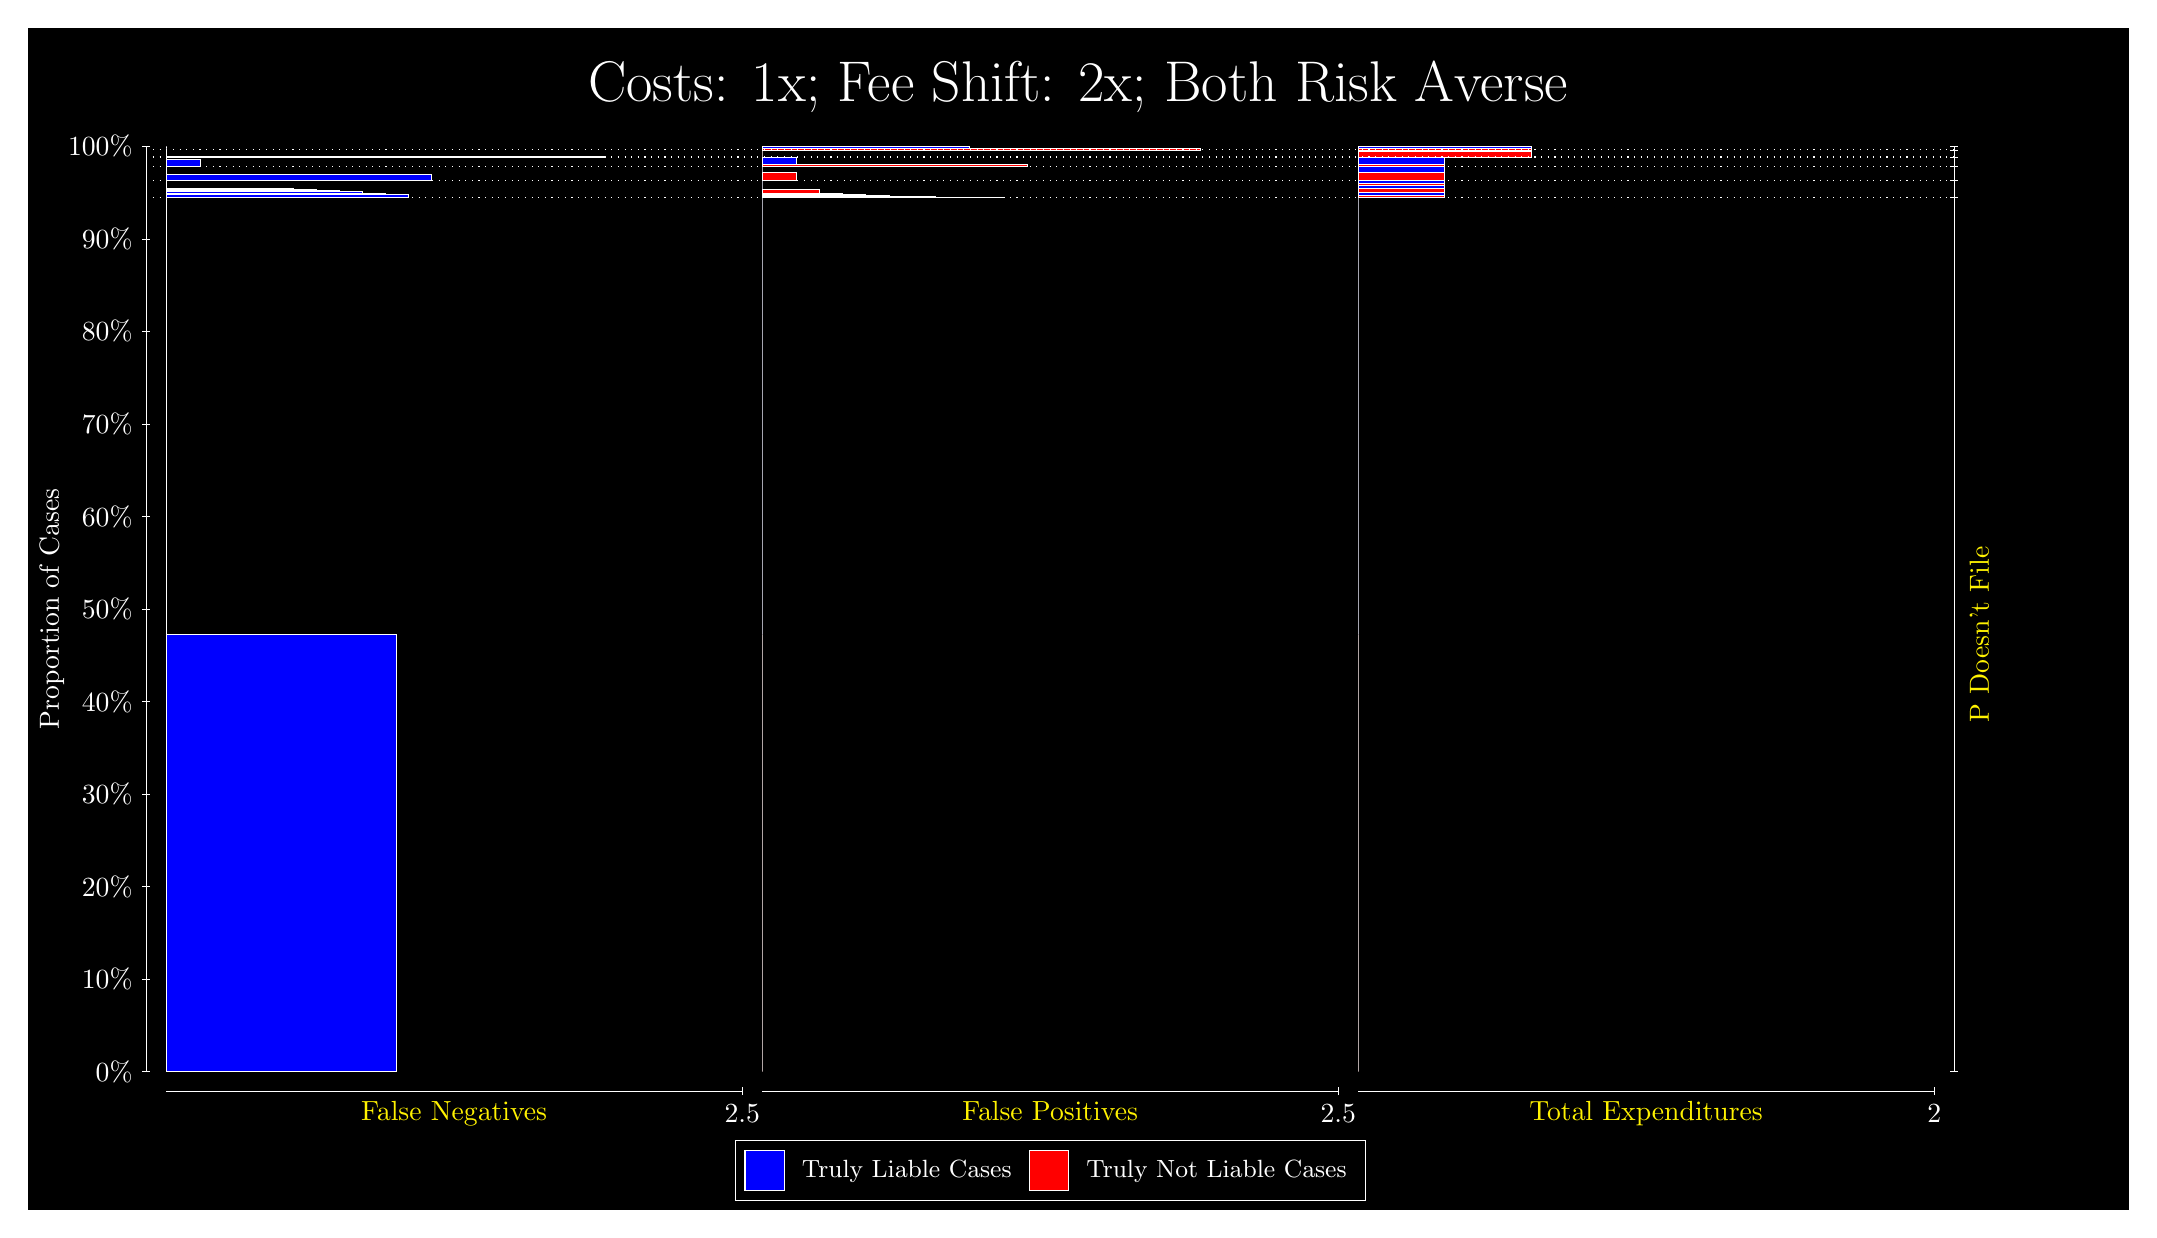
\begin{tikzpicture}
\draw[fill=black] (0,0) rectangle (26.667,15);
\draw[text=white] (0,13.5) rectangle (26.667,15) node[midway] {\huge Costs: 1x; Fee Shift: 2x; Both Risk Averse};
\draw[white, very thin] (1.5,1.75) -- (1.5,13.5);
\node[rotate=90, text=white, anchor=center] at (0.3, 7.625) {Proportion of Cases};
\draw[white, very thin] (1.45,1.75) -- (1.55,1.75);
\node[text=white, anchor=east] at (1.45, 1.75) {0\%};
\draw[white, very thin] (1.45,2.925) -- (1.55,2.925);
\node[text=white, anchor=east] at (1.45, 2.925) {10\%};
\draw[white, very thin] (1.45,4.1) -- (1.55,4.1);
\node[text=white, anchor=east] at (1.45, 4.1) {20\%};
\draw[white, very thin] (1.45,5.275) -- (1.55,5.275);
\node[text=white, anchor=east] at (1.45, 5.275) {30\%};
\draw[white, very thin] (1.45,6.45) -- (1.55,6.45);
\node[text=white, anchor=east] at (1.45, 6.45) {40\%};
\draw[white, very thin] (1.45,7.625) -- (1.55,7.625);
\node[text=white, anchor=east] at (1.45, 7.625) {50\%};
\draw[white, very thin] (1.45,8.8) -- (1.55,8.8);
\node[text=white, anchor=east] at (1.45, 8.8) {60\%};
\draw[white, very thin] (1.45,9.975) -- (1.55,9.975);
\node[text=white, anchor=east] at (1.45, 9.975) {70\%};
\draw[white, very thin] (1.45,11.15) -- (1.55,11.15);
\node[text=white, anchor=east] at (1.45, 11.15) {80\%};
\draw[white, very thin] (1.45,12.325) -- (1.55,12.325);
\node[text=white, anchor=east] at (1.45, 12.325) {90\%};
\draw[white, very thin] (1.45,13.5) -- (1.55,13.5);
\node[text=white, anchor=east] at (1.45, 13.5) {100\%};

\draw[white, very thin] (24.457,1.75) -- (24.457,13.5);
\draw[white, very thin] (24.407,1.75) -- (24.507,1.75);
\node[anchor=west] at (24.407, 1.75) {};
\draw[white, very thin] (24.407,12.852) -- (24.507,12.852);
\node[anchor=west] at (24.407, 12.852) {};
\draw[white, very thin] (24.407,13.07) -- (24.507,13.07);
\node[anchor=west] at (24.407, 13.07) {};
\draw[white, very thin] (24.407,13.245) -- (24.507,13.245);
\node[anchor=west] at (24.407, 13.245) {};
\draw[white, very thin] (24.407,13.364) -- (24.507,13.364);
\node[anchor=west] at (24.407, 13.364) {};
\draw[white, very thin] (24.407,13.456) -- (24.507,13.456);
\node[anchor=west] at (24.407, 13.456) {};
\draw[white, very thin] (24.407,13.5) -- (24.507,13.5);
\node[anchor=west] at (24.407, 13.5) {};

\draw[white, very thin, fill=blue] (1.75,1.75) rectangle (4.6775,7.3008);
\draw[white, very thin, fill=red] (1.75,7.3008) rectangle (1.75,12.852);
\draw[white, very thin, fill=blue] (1.75,12.852) rectangle (4.8239,12.886);
\draw[white, very thin, fill=blue] (1.75,12.886) rectangle (4.5312,12.899);
\draw[white, very thin, fill=blue] (1.75,12.899) rectangle (4.2384,12.927);
\draw[white, very thin, fill=blue] (1.75,12.927) rectangle (3.9457,12.944);
\draw[white, very thin, fill=blue] (1.75,12.944) rectangle (3.6529,12.96);
\draw[white, very thin, fill=blue] (1.75,12.96) rectangle (3.3602,12.964);
\draw[white, very thin, fill=blue] (1.75,12.964) rectangle (3.0674,12.967);
\draw[white, very thin, fill=blue] (1.75,12.967) rectangle (2.7746,12.968);
\draw[white, very thin, fill=blue] (1.75,12.968) rectangle (2.4819,12.97);
\draw[white, very thin, fill=red] (1.75,12.97) rectangle (1.75,13.07);
\draw[white, very thin, fill=blue] (1.75,13.07) rectangle (5.1167,13.144);
\draw[white, very thin, fill=red] (1.75,13.144) rectangle (1.75,13.245);
\draw[white, very thin, fill=blue] (1.75,13.245) rectangle (2.1891,13.333);
\draw[white, very thin, fill=red] (1.75,13.333) rectangle (1.75,13.364);
\draw[white, very thin, fill=blue] (1.75,13.364) rectangle (7.3123,13.378);
\draw[white, very thin, fill=red] (1.75,13.378) rectangle (1.75,13.456);
\draw[white, very thin, fill=red] (1.75,13.456) rectangle (1.75,13.47);
\draw[white, very thin, fill=blue] (1.75,13.47) rectangle (1.75,13.5);
\draw[white, very thin, fill=red] (9.3189,1.75) rectangle (9.3189,7.3009);
\draw[white, very thin, fill=blue] (9.3189,7.3009) rectangle (9.3189,12.852);
\draw[white, very thin, fill=red] (9.3189,12.852) rectangle (12.393,12.853);
\draw[white, very thin, fill=red] (9.3189,12.853) rectangle (12.1,12.855);
\draw[white, very thin, fill=red] (9.3189,12.855) rectangle (11.807,12.857);
\draw[white, very thin, fill=red] (9.3189,12.857) rectangle (11.515,12.86);
\draw[white, very thin, fill=red] (9.3189,12.86) rectangle (11.222,12.87);
\draw[white, very thin, fill=red] (9.3189,12.87) rectangle (10.929,12.876);
\draw[white, very thin, fill=red] (9.3189,12.876) rectangle (10.929,12.878);
\draw[white, very thin, fill=red] (9.3189,12.878) rectangle (10.636,12.893);
\draw[white, very thin, fill=red] (9.3189,12.893) rectangle (10.344,12.9);
\draw[white, very thin, fill=red] (9.3189,12.9) rectangle (10.051,12.952);
\draw[white, very thin, fill=blue] (9.3189,12.952) rectangle (9.4652,12.953);
\draw[white, very thin, fill=blue] (9.3189,12.953) rectangle (9.3189,13.07);
\draw[white, very thin, fill=red] (9.3189,13.07) rectangle (9.758,13.171);
\draw[white, very thin, fill=blue] (9.3189,13.171) rectangle (9.3189,13.245);
\draw[white, very thin, fill=red] (9.3189,13.245) rectangle (12.686,13.276);
\draw[white, very thin, fill=blue] (9.3189,13.276) rectangle (9.758,13.364);
\draw[white, very thin, fill=red] (9.3189,13.364) rectangle (9.3189,13.442);
\draw[white, very thin, fill=blue] (9.3189,13.442) rectangle (9.3189,13.456);
\draw[white, very thin, fill=red] (9.3189,13.456) rectangle (14.881,13.47);
\draw[white, very thin, fill=blue] (9.3189,13.47) rectangle (11.954,13.5);
\draw[white, very thin, fill=red] (16.888,1.75) rectangle (16.888,7.3009);
\draw[white, very thin, fill=blue] (16.888,7.3009) rectangle (16.888,12.852);
\draw[white, very thin, fill=red] (16.888,12.852) rectangle (17.986,12.876);
\draw[white, very thin, fill=blue] (16.888,12.876) rectangle (17.986,12.917);
\draw[white, very thin, fill=red] (16.888,12.917) rectangle (17.986,12.969);
\draw[white, very thin, fill=blue] (16.888,12.969) rectangle (17.986,13.002);
\draw[white, very thin, fill=red] (16.888,13.002) rectangle (17.986,13.026);
\draw[white, very thin, fill=blue] (16.888,13.026) rectangle (17.986,13.07);
\draw[white, very thin, fill=red] (16.888,13.07) rectangle (17.986,13.171);
\draw[white, very thin, fill=blue] (16.888,13.171) rectangle (17.986,13.245);
\draw[white, very thin, fill=red] (16.888,13.245) rectangle (17.986,13.276);
\draw[white, very thin, fill=blue] (16.888,13.276) rectangle (17.986,13.364);
\draw[white, very thin, fill=red] (16.888,13.364) rectangle (19.083,13.442);
\draw[white, very thin, fill=blue] (16.888,13.442) rectangle (19.083,13.456);
\draw[white, very thin, fill=red] (16.888,13.456) rectangle (19.083,13.47);
\draw[white, very thin, fill=blue] (16.888,13.47) rectangle (19.083,13.5);
\draw[white, dotted] (1.5,12.852) -- (24.457,12.852);
\draw[white, dotted] (1.5,13.07) -- (24.457,13.07);
\draw[white, dotted] (1.5,13.245) -- (24.457,13.245);
\draw[white, dotted] (1.5,13.364) -- (24.457,13.364);
\draw[white, dotted] (1.5,13.456) -- (24.457,13.456);
\draw[white, very thin] (1.75,1.5) -- (9.0689,1.5);
\node[text=yellow, anchor=north] at (5.4094, 1.5) {False Negatives};
\draw[white, very thin] (9.0689,1.45) -- (9.0689,1.55);
\node[text=white, anchor=north] at (9.0689, 1.45) {2.5};

\draw[white, very thin] (9.3189,1.5) -- (16.638,1.5);
\node[text=yellow, anchor=north] at (12.978, 1.5) {False Positives};
\draw[white, very thin] (16.638,1.45) -- (16.638,1.55);
\node[text=white, anchor=north] at (16.638, 1.45) {2.5};

\draw[white, very thin] (16.888,1.5) -- (24.207,1.5);
\node[text=yellow, anchor=north] at (20.547, 1.5) {Total Expenditures};
\draw[white, very thin] (24.207,1.45) -- (24.207,1.55);
\node[text=white, anchor=north] at (24.207, 1.45) {2};

\node[text=yellow, centered, rotate=90] at (24.777, 7.3009) {P Doesn't File};






\draw (12.978300999999998,1.5) node[draw=none] (baseCoordinate) {};
\begin{scope}[align=center]
        \matrix[scale=0.5, draw=white, below=0.5cm of baseCoordinate, nodes={draw}, column sep=0.1cm]{
            \node[rectangle, draw, minimum width=0.5cm, minimum height=0.5cm, fill=blue] {}; &
            \node[draw=none, font=\small, text=white] (B) {Truly Liable Cases}; &
            \node[rectangle, draw, minimum width=0.5cm, minimum height=0.5cm, fill=red] {}; &
            \node[draw=none, font=\small, text=white] (B) {Truly Not Liable Cases}; \\
            };
\end{scope}

\end{tikzpicture}
\end{document}